%% knit("quad-rig_catch_comparison.Rnw")

\documentclass[12pt]{article}\usepackage[]{graphicx}\usepackage[]{color}
%% maxwidth is the original width if it is less than linewidth
%% otherwise use linewidth (to make sure the graphics do not exceed the margin)
\makeatletter
\def\maxwidth{ %
  \ifdim\Gin@nat@width>\linewidth
    \linewidth
  \else
    \Gin@nat@width
  \fi
}
\makeatother

\definecolor{fgcolor}{rgb}{0.345, 0.345, 0.345}
\newcommand{\hlnum}[1]{\textcolor[rgb]{0.686,0.059,0.569}{#1}}%
\newcommand{\hlstr}[1]{\textcolor[rgb]{0.192,0.494,0.8}{#1}}%
\newcommand{\hlcom}[1]{\textcolor[rgb]{0.678,0.584,0.686}{\textit{#1}}}%
\newcommand{\hlopt}[1]{\textcolor[rgb]{0,0,0}{#1}}%
\newcommand{\hlstd}[1]{\textcolor[rgb]{0.345,0.345,0.345}{#1}}%
\newcommand{\hlkwa}[1]{\textcolor[rgb]{0.161,0.373,0.58}{\textbf{#1}}}%
\newcommand{\hlkwb}[1]{\textcolor[rgb]{0.69,0.353,0.396}{#1}}%
\newcommand{\hlkwc}[1]{\textcolor[rgb]{0.333,0.667,0.333}{#1}}%
\newcommand{\hlkwd}[1]{\textcolor[rgb]{0.737,0.353,0.396}{\textbf{#1}}}%

\usepackage{framed}
\makeatletter
\newenvironment{kframe}{%
 \def\at@end@of@kframe{}%
 \ifinner\ifhmode%
  \def\at@end@of@kframe{\end{minipage}}%
  \begin{minipage}{\columnwidth}%
 \fi\fi%
 \def\FrameCommand##1{\hskip\@totalleftmargin \hskip-\fboxsep
 \colorbox{shadecolor}{##1}\hskip-\fboxsep
     % There is no \\@totalrightmargin, so:
     \hskip-\linewidth \hskip-\@totalleftmargin \hskip\columnwidth}%
 \MakeFramed {\advance\hsize-\width
   \@totalleftmargin\z@ \linewidth\hsize
   \@setminipage}}%
 {\par\unskip\endMakeFramed%
 \at@end@of@kframe}
\makeatother

\definecolor{shadecolor}{rgb}{.97, .97, .97}
\definecolor{messagecolor}{rgb}{0, 0, 0}
\definecolor{warningcolor}{rgb}{1, 0, 1}
\definecolor{errorcolor}{rgb}{1, 0, 0}
\newenvironment{knitrout}{}{} % an empty environment to be redefined in TeX

\usepackage{alltt}
\usepackage{times}
\usepackage{hyperref}
\usepackage{natbib}
\hypersetup{pdfpagemode=UseNone} % don't show bookmarks on initial view
\hypersetup{colorlinks, urlcolor={blue}}

% revise margins
\setlength{\headheight}{0.0in}
\setlength{\topmargin}{0.0in}
\setlength{\headsep}{0.0in}
\setlength{\textheight}{8.65in}
\setlength{\footskip}{0.35in}
\setlength{\oddsidemargin}{0.0in}
\setlength{\evensidemargin}{0.0in}
\setlength{\textwidth}{6.5in}

\setlength{\parskip}{6pt}
\setlength{\parindent}{0pt}

\title{A preliminary model for Quad-Rig catch comparison}
\author{Updated to include additional trial data}
\date{}
\IfFileExists{upquote.sty}{\usepackage{upquote}}{}
\begin{document}



\maketitle
Methods for twin-rig catch comparison analysis are set out in \citet{Holst:Reville:2009}. Here, this model is preliminarily extended to greater than 2 cod-ends, in particular we focus on the quad-rig with 4 cod-ends. All treatment of the data is included as in a tutorial, which can be used as a basis for capacity building in the analysis of gear technology trials.

\section{Data}
The data used for this example come from the July 2014 diamond cod-end mesh size trials conducted by BIM aboard MFV Celtic Warrior II on the Smalls grounds. The data are read into R and processed as follows:

\begin{knitrout}\footnotesize
\definecolor{shadecolor}{rgb}{0.969, 0.969, 0.969}\color{fgcolor}\begin{kframe}
\begin{alltt}
\hlkwd{library}\hlstd{(gdata)}

\hlstd{neph.dat} \hlkwb{<-} \hlkwd{read.xls}\hlstd{(}\hlstr{"../data/Celtic Warrior Diamond mesh July 2014 Celtic Sea.xls"}\hlstd{,}
                     \hlkwc{sheet} \hlstd{=} \hlstr{"Nephrops Lengths"}\hlstd{,}
                     \hlkwc{stringsAsFactors} \hlstd{=} \hlnum{FALSE}\hlstd{)}

\hlcom{## remove Haul 22, as no recordings for 90mm }
\hlstd{neph.dat} \hlkwb{<-} \hlkwd{subset}\hlstd{(neph.dat, HAUL} \hlopt{!=} \hlnum{22}\hlstd{)}

\hlcom{## Show the first 2 rows}
\hlkwd{head}\hlstd{(neph.dat,} \hlnum{2}\hlstd{)}
\end{alltt}
\begin{verbatim}
##           Vessel       DATE HAUL COMPARTMENT Mesh.Size  SPECIES
## 1 Celtic Warrior 2014-07-19    1     Control      70mm Nephrops
## 2 Celtic Warrior 2014-07-19    1     Control      70mm Nephrops
##   Carapace.Length..mm.. COUNT SUBSRATIO
## 1                    16     1         1
## 2                    17    11         1
\end{verbatim}
\begin{alltt}
\hlcom{## Change the carapace length name}
\hlkwd{names}\hlstd{(neph.dat)[}\hlkwd{names}\hlstd{(neph.dat)} \hlopt{==} \hlstr{"Carapace.Length..mm.."}\hlstd{]} \hlkwb{<-} \hlstr{"Carapace.Length"}

\hlcom{## Make the "HAUL" variable character}
\hlstd{neph.dat}\hlopt{$}\hlstd{HAUL} \hlkwb{<-} \hlkwd{paste}\hlstd{(}\hlstr{"H"}\hlstd{, neph.dat}\hlopt{$}\hlstd{HAUL,} \hlkwc{sep} \hlstd{=}\hlstr{""}\hlstd{)}

\hlcom{## make some factor variables used in the analyses}
\hlstd{neph.dat}\hlopt{$}\hlstd{fHAUL} \hlkwb{<-} \hlkwd{factor}\hlstd{(neph.dat}\hlopt{$}\hlstd{HAUL,} \hlkwc{levels} \hlstd{=} \hlkwd{unique}\hlstd{(neph.dat}\hlopt{$}\hlstd{HAUL))}
\hlstd{neph.dat}\hlopt{$}\hlstd{fMesh.Size} \hlkwb{<-} \hlkwd{factor}\hlstd{(neph.dat}\hlopt{$}\hlstd{Mesh.Size,} \hlkwc{levels} \hlstd{=} \hlkwd{unique}\hlstd{(neph.dat}\hlopt{$}\hlstd{Mesh.Size))}

\hlcom{## remove observations above 99th and below 1th length percentile}
\hlcom{## these can be highly influential on the fits}
\hlstd{neph.dat} \hlkwb{<-} \hlkwd{subset}\hlstd{(neph.dat, Carapace.Length} \hlopt{<} \hlkwd{quantile}\hlstd{(Carapace.Length,} \hlnum{0.99}\hlstd{)} \hlopt{&}
                   \hlstd{Carapace.Length} \hlopt{>} \hlkwd{quantile}\hlstd{(Carapace.Length,} \hlnum{0.01}\hlstd{)}
                   \hlstd{)}
\end{alltt}
\end{kframe}
\end{knitrout}

Prepare the data for a multinomial fit.  

\begin{knitrout}\footnotesize
\definecolor{shadecolor}{rgb}{0.969, 0.969, 0.969}\color{fgcolor}\begin{kframe}
\begin{alltt}
\hlcom{## get count per length bin per haul by mesh size}
\hlcom{## using the reshape package (makes it easier to process data)}
\hlkwd{library}\hlstd{(reshape)}

\hlcom{## variables to keep }
\hlstd{vars2keep} \hlkwb{<-} \hlkwd{c}\hlstd{(}\hlstr{"fMesh.Size"}\hlstd{,} \hlstr{"Carapace.Length"}\hlstd{,} \hlstr{"fHAUL"}\hlstd{,} \hlstr{"COUNT"}\hlstd{)}

\hlcom{## melt the data frame}
\hlstd{neph.melt} \hlkwb{<-} \hlkwd{melt}\hlstd{(neph.dat[, vars2keep],}
                  \hlkwc{id} \hlstd{=} \hlkwd{c}\hlstd{(}\hlstr{"fMesh.Size"}\hlstd{,} \hlstr{"Carapace.Length"}\hlstd{,} \hlstr{"fHAUL"}\hlstd{))}

\hlcom{## re-form the dataframe in required format }
\hlstd{neph.cast} \hlkwb{<-} \hlkwd{cast}\hlstd{(neph.melt, Carapace.Length} \hlopt{+} \hlstd{fHAUL} \hlopt{~} \hlstd{fMesh.Size}  \hlopt{+} \hlstd{variable)}
\hlstd{neph.cast} \hlkwb{<-} \hlstd{neph.cast[}\hlkwd{order}\hlstd{(neph.cast}\hlopt{$}\hlstd{fHAUL, neph.cast}\hlopt{$}\hlstd{Carapace.Length), ]}
\hlstd{neph.cast[}\hlkwd{is.na}\hlstd{(neph.cast)]} \hlkwb{<-} \hlnum{0}

\hlcom{## show the first few rows}
\hlkwd{head}\hlstd{(neph.cast,} \hlnum{2}\hlstd{)}
\end{alltt}
\begin{verbatim}
##    Carapace.Length fHAUL 70mm_COUNT 80mm_COUNT 90mm_COUNT 100mm_COUNT
## 1               15    H1          0          2          1           0
## 24              16    H1          1          3          9           1
\end{verbatim}
\begin{alltt}
\hlcom{## format the subsampling ratio similarly}
\hlstd{vars2keep} \hlkwb{<-} \hlkwd{c}\hlstd{(}\hlstr{"fMesh.Size"}\hlstd{,} \hlstr{"fHAUL"}\hlstd{,} \hlstr{"SUBSRATIO"}\hlstd{)}

\hlstd{subs.melt} \hlkwb{<-} \hlkwd{melt}\hlstd{(}\hlkwd{unique}\hlstd{(neph.dat[, vars2keep]),} \hlkwc{id} \hlstd{=} \hlkwd{c}\hlstd{(}\hlstr{"fMesh.Size"}\hlstd{,} \hlstr{"fHAUL"}\hlstd{))}

\hlstd{subs.cast} \hlkwb{<-} \hlkwd{cast}\hlstd{(subs.melt, fHAUL}  \hlopt{~} \hlstd{fMesh.Size} \hlopt{+} \hlstd{variable)}

\hlcom{## merge counts and subsampling ratio back together }
\hlstd{neph.cast} \hlkwb{<-} \hlkwd{merge}\hlstd{(neph.cast, subs.cast,} \hlkwc{by} \hlstd{=} \hlstr{"fHAUL"}\hlstd{,} \hlkwc{all.x} \hlstd{=} \hlnum{TRUE}\hlstd{)}

\hlcom{## show first few lines}
\hlkwd{head}\hlstd{(neph.cast,} \hlnum{2}\hlstd{)}
\end{alltt}
\begin{verbatim}
##   fHAUL Carapace.Length 70mm_COUNT 80mm_COUNT 90mm_COUNT 100mm_COUNT
## 1    H1              15          0          2          1           0
## 2    H1              16          1          3          9           1
##   70mm_SUBSRATIO 80mm_SUBSRATIO 90mm_SUBSRATIO 100mm_SUBSRATIO
## 1              1              1              1               1
## 2              1              1              1               1
\end{verbatim}
\begin{alltt}
\hlcom{## Extract the matrix of counts}
\hlstd{count.vars} \hlkwb{<-} \hlkwd{c}\hlstd{(}\hlstr{"70mm_COUNT"}\hlstd{,} \hlstr{"80mm_COUNT"}\hlstd{,} \hlstr{"90mm_COUNT"}\hlstd{,} \hlstr{"100mm_COUNT"}\hlstd{)}

\hlstd{neph.count.mat} \hlkwb{<-} \hlkwd{as.matrix}\hlstd{(neph.cast[, count.vars])}

\hlkwd{colnames}\hlstd{(neph.count.mat)} \hlkwb{<-} \hlkwd{c}\hlstd{(}\hlstr{"70mm_COUNT"}\hlstd{,} \hlstr{"80mm_COUNT"}\hlstd{,} \hlstr{"90mm_COUNT"}\hlstd{,}
                              \hlstr{"100mm_COUNT"}\hlstd{)}

\hlcom{## Extract the matrix of subsampling ratios}
\hlstd{subsratio.vars} \hlkwb{<-} \hlkwd{c}\hlstd{(}\hlstr{"70mm_SUBSRATIO"}\hlstd{,} \hlstr{"80mm_SUBSRATIO"}\hlstd{,} \hlstr{"90mm_SUBSRATIO"}\hlstd{,}
                    \hlstr{"100mm_SUBSRATIO"}\hlstd{)}

\hlstd{subsratio.mat} \hlkwb{<-} \hlkwd{as.matrix}\hlstd{(neph.cast[, subsratio.vars])}

\hlcom{## Create the offset (NEED TO CHECK THIS)}
\hlstd{offset.mat} \hlkwb{<-} \hlkwd{log}\hlstd{(}\hlkwd{apply}\hlstd{(subsratio.mat,} \hlnum{2}\hlstd{,} \hlkwc{FUN} \hlstd{=}
                        \hlkwa{function}\hlstd{(}\hlkwc{zz}\hlstd{)\{zz}\hlopt{/}\hlstd{subsratio.mat[,}\hlnum{1}\hlstd{]\}))}
\end{alltt}
\end{kframe}
\end{knitrout}

Plot the data 
\begin{knitrout}\footnotesize
\definecolor{shadecolor}{rgb}{0.969, 0.969, 0.969}\color{fgcolor}\begin{kframe}
\begin{alltt}
\hlkwd{library}\hlstd{(ggplot2)}

\hlcom{## Get the proportions}
\hlstd{count.mesh} \hlkwb{<-} \hlkwd{as.matrix}\hlstd{(neph.cast[, count.vars])}

\hlstd{prop.mesh} \hlkwb{<-} \hlkwd{prop.table}\hlstd{(count.mesh,} \hlkwc{margin} \hlstd{=} \hlnum{1}\hlstd{)}

\hlstd{m} \hlkwb{<-} \hlkwd{dim}\hlstd{(prop.mesh)[}\hlnum{1}\hlstd{]}

\hlcom{## make a dataframe of the proportions for ggplot}
\hlstd{prop.mesh.df} \hlkwb{<-} \hlkwd{data.frame}\hlstd{(}
                  \hlkwc{Mesh.Size} \hlstd{=} \hlkwd{factor}\hlstd{(}\hlkwd{rep}\hlstd{(}\hlkwd{c}\hlstd{(}\hlstr{"70mm"}\hlstd{,} \hlstr{"80mm"}\hlstd{,} \hlstr{"90mm"}\hlstd{,} \hlstr{"100mm"}\hlstd{),}
                    \hlkwc{each} \hlstd{= m),} \hlkwc{levels} \hlstd{=} \hlkwd{c}\hlstd{(}\hlstr{"70mm"}\hlstd{,} \hlstr{"80mm"}\hlstd{,} \hlstr{"90mm"}\hlstd{,} \hlstr{"100mm"}\hlstd{)),}
                  \hlkwc{Carapace.Length} \hlstd{=} \hlkwd{rep}\hlstd{(neph.cast}\hlopt{$}\hlstd{Carapace.Length,} \hlkwc{times} \hlstd{=} \hlnum{4}\hlstd{),}
                  \hlkwc{proportion} \hlstd{=} \hlkwd{c}\hlstd{(prop.mesh),}
                  \hlkwc{count} \hlstd{=} \hlkwd{c}\hlstd{(count.mesh))}

\hlkwd{ggplot}\hlstd{(prop.mesh.df,} \hlkwd{aes}\hlstd{(}\hlkwc{x} \hlstd{= Carapace.Length,} \hlkwc{y} \hlstd{= proportion))} \hlopt{+}
  \hlkwd{geom_point}\hlstd{(}\hlkwc{colour} \hlstd{=} \hlstr{"#F8766D"}\hlstd{,} \hlkwc{alpha} \hlstd{=} \hlnum{0.2}\hlstd{,} \hlkwd{aes}\hlstd{(}\hlkwc{size} \hlstd{=} \hlkwd{log}\hlstd{(count)))} \hlopt{+}
  \hlkwd{facet_wrap}\hlstd{(}\hlopt{~} \hlstd{Mesh.Size)} \hlopt{+} \hlkwd{ylab}\hlstd{(}\hlstr{"Proportion of Nephrops per cod-end"}\hlstd{)}
\end{alltt}
\end{kframe}\begin{figure}
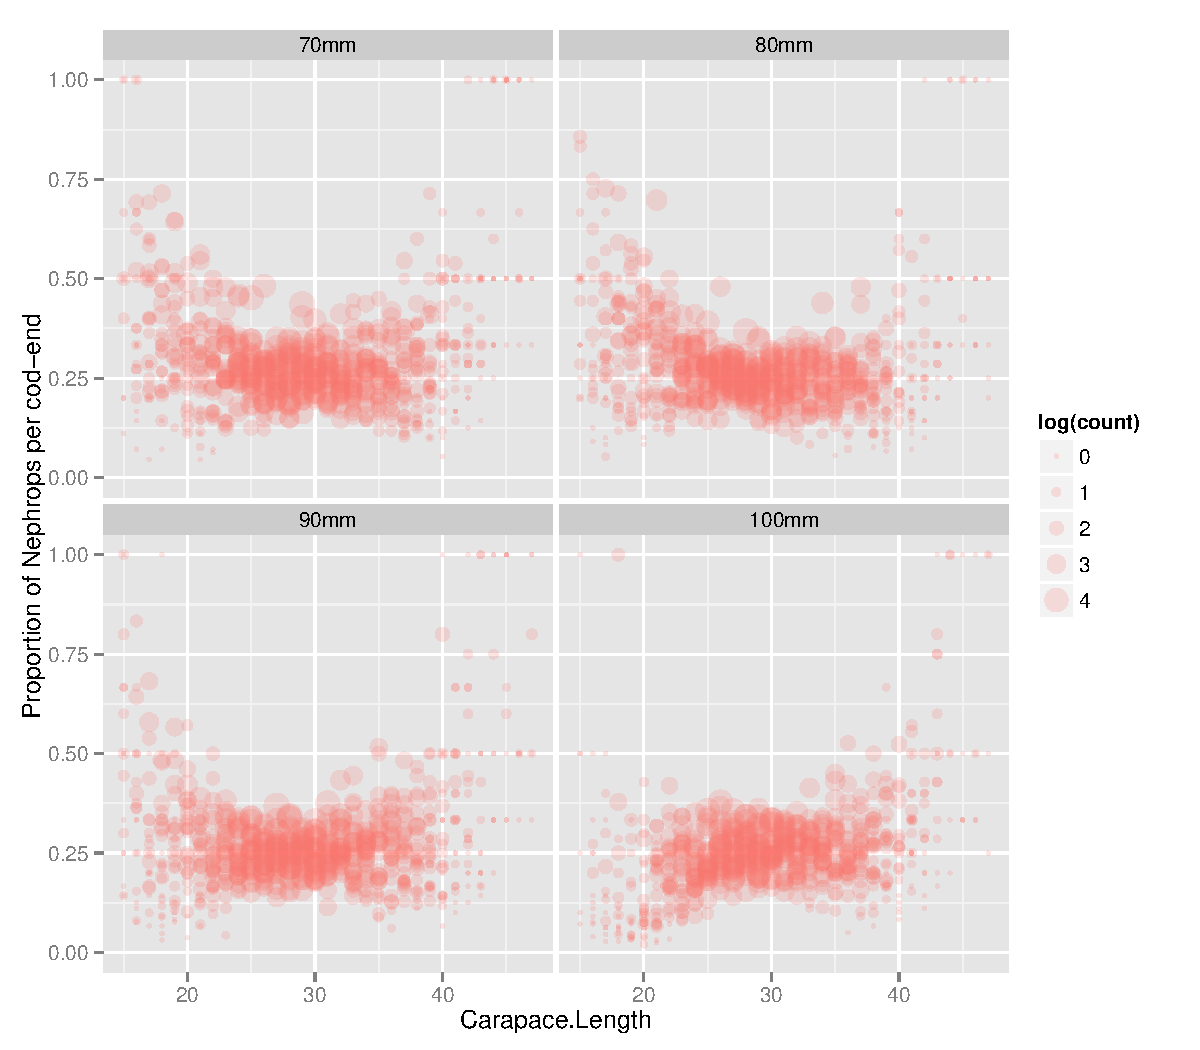
\includegraphics[width=\maxwidth]{figure/unnamed-chunk-4-1} \caption[Proportion of Nephrops catch retained per haul]{Proportion of Nephrops catch retained per haul. Each point represents the proportion of the Nephrops catch (in number) per haul and length class retained in a given cod-end (70mm, 80mm, 90mm, or 100mm). The size of the point is proportional to the log of the count.}\label{fig:unnamed-chunk-4}
\end{figure}


\end{knitrout}

\section{Model}
The model we focus on is the multinomial, which is a generalization of the binomial to cases with more than two categories (here 4 categories: 70mm, 80mm, 90mm, 100mm). Under the assumption that each net fishes the same, we would expect 25\% of the catch to be retained in each net. We can test that hypothesis.

\begin{knitrout}\footnotesize
\definecolor{shadecolor}{rgb}{0.969, 0.969, 0.969}\color{fgcolor}\begin{kframe}
\begin{alltt}
\hlkwd{library}\hlstd{(nnet)}

\hlcom{## First fit is constant proportions}
\hlcom{## not accounting for length}

\hlstd{mnom0} \hlkwb{<-} \hlkwd{multinom}\hlstd{(neph.count.mat} \hlopt{~} \hlnum{1} \hlopt{+} \hlkwd{offset}\hlstd{(offset.mat))}
\end{alltt}
\begin{verbatim}
## # weights:  24 (3 variable)
## initial  value 65833.303791 
## final  value 65796.538161 
## converged
\end{verbatim}
\begin{alltt}
\hlcom{## include carapace length }
\hlcom{## first scale it to range between zero and one}
\hlstd{max.length} \hlkwb{<-} \hlkwd{max}\hlstd{(neph.cast}\hlopt{$}\hlstd{Carapace.Length)}
\hlstd{neph.cast}\hlopt{$}\hlstd{prop.Carapace.Length} \hlkwb{<-} \hlstd{neph.cast}\hlopt{$}\hlstd{Carapace.Length}\hlopt{/}\hlstd{max.length}

\hlcom{## Extend to third order polynomial (based on AIC and BIC)}
\hlstd{neph.cast}\hlopt{$}\hlstd{prop.Carapace.Length2} \hlkwb{<-} \hlstd{neph.cast}\hlopt{$}\hlstd{prop.Carapace.Length}\hlopt{^}\hlnum{2}
\hlstd{neph.cast}\hlopt{$}\hlstd{prop.Carapace.Length3} \hlkwb{<-} \hlstd{neph.cast}\hlopt{$}\hlstd{prop.Carapace.Length}\hlopt{^}\hlnum{3}

\hlcom{## }
\hlstd{mnom.length} \hlkwb{<-} \hlkwd{multinom}\hlstd{(neph.count.mat} \hlopt{~}
                        \hlstd{prop.Carapace.Length} \hlopt{+} \hlstd{prop.Carapace.Length2} \hlopt{+} \hlstd{prop.Carapace.Length3} \hlopt{+}
                        \hlkwd{offset}\hlstd{(offset.mat),} \hlkwc{data} \hlstd{= neph.cast)}
\end{alltt}
\begin{verbatim}
## # weights:  36 (12 variable)
## initial  value 65833.303791 
## iter  10 value 65574.013563
## iter  20 value 65540.974075
## final  value 65538.628411 
## converged
\end{verbatim}
\begin{alltt}
\hlkwd{AIC}\hlstd{(mnom0, mnom.length)}
\end{alltt}
\begin{verbatim}
##             df      AIC
## mnom0        3 131599.1
## mnom.length 12 131101.3
\end{verbatim}
\end{kframe}
\end{knitrout}

Get predictions for the fitted model (note this is long-winded here but will be better coded for more than the preliminary example).

\begin{knitrout}\footnotesize
\definecolor{shadecolor}{rgb}{0.969, 0.969, 0.969}\color{fgcolor}\begin{kframe}
\begin{alltt}
\hlcom{## get predictions manually}
\hlcom{## CIs not defined in multinomial context but let's try}

\hlcom{## fit coefficients}
\hlstd{beta.mu} \hlkwb{<-} \hlkwd{c}\hlstd{(}\hlkwd{t}\hlstd{(}\hlkwd{coef}\hlstd{(mnom.length)))}

\hlcom{## fit coefficient variance covariance matrix}
\hlstd{Sigma} \hlkwb{<-} \hlkwd{vcov}\hlstd{(mnom.length)}

\hlcom{## number of lengths to predict for}
\hlstd{nlength} \hlkwb{<-} \hlnum{100}
\hlstd{pred.prop.length} \hlkwb{<-} \hlkwd{seq}\hlstd{(}\hlkwd{min}\hlstd{(neph.cast}\hlopt{$}\hlstd{prop.Carapace.Length),}
                        \hlkwd{max}\hlstd{(neph.cast}\hlopt{$}\hlstd{prop.Carapace.Length),} \hlkwc{length} \hlstd{=} \hlnum{100}\hlstd{)}

\hlstd{pred.length} \hlkwb{<-} \hlkwd{seq}\hlstd{(}\hlkwd{min}\hlstd{(neph.cast}\hlopt{$}\hlstd{Carapace.Length),}
                        \hlkwd{max}\hlstd{(neph.cast}\hlopt{$}\hlstd{Carapace.Length),} \hlkwc{length} \hlstd{=} \hlnum{100}\hlstd{)}

\hlcom{## model matrix}
\hlstd{X} \hlkwb{<-} \hlkwd{cbind}\hlstd{(}\hlnum{1}\hlstd{, pred.prop.length, pred.prop.length}\hlopt{^}\hlnum{2}\hlstd{, pred.prop.length}\hlopt{^}\hlnum{3}\hlstd{)}

\hlcom{## number of times to resample predictions to get CIs}
\hlstd{nresamp} \hlkwb{<-} \hlnum{100}
\hlstd{pred.array} \hlkwb{<-} \hlkwd{array}\hlstd{(}\hlnum{NA}\hlstd{,} \hlkwc{dim} \hlstd{=} \hlkwd{c}\hlstd{(nlength,} \hlnum{4}\hlstd{, nresamp))}

\hlcom{## package to draw from multivariate normal }
\hlkwd{library}\hlstd{(mvtnorm)}

\hlkwa{for}\hlstd{(i} \hlkwa{in} \hlnum{1}\hlopt{:}\hlstd{nresamp)\{}
  \hlcom{## print(i)}
  \hlstd{beta} \hlkwb{<-} \hlkwd{matrix}\hlstd{(}\hlkwd{rmvnorm}\hlstd{(}\hlnum{1}\hlstd{,} \hlkwc{mean} \hlstd{= beta.mu,} \hlkwc{sigma} \hlstd{= Sigma),}
                 \hlkwc{nrow} \hlstd{=} \hlnum{3}\hlstd{,} \hlkwc{byrow} \hlstd{=} \hlnum{TRUE}\hlstd{)}
  \hlstd{p80} \hlkwb{<-} \hlkwd{exp}\hlstd{(X} \hlopt \hlkwd{matrix}\hlstd{(beta[}\hlnum{1}\hlstd{,]))}\hlopt{/}\hlstd{(}\hlnum{1} \hlopt{+} \hlkwd{rowSums}\hlstd{(}\hlkwd{exp}\hlstd{(X} \hlopt \hlkwd{t}\hlstd{(beta))))}
  \hlstd{p90} \hlkwb{<-} \hlkwd{exp}\hlstd{(X} \hlopt \hlkwd{matrix}\hlstd{(beta[}\hlnum{2}\hlstd{,]))}\hlopt{/}\hlstd{(}\hlnum{1} \hlopt{+} \hlkwd{rowSums}\hlstd{(}\hlkwd{exp}\hlstd{(X} \hlopt \hlkwd{t}\hlstd{(beta))))}
  \hlstd{p100} \hlkwb{<-} \hlkwd{exp}\hlstd{(X} \hlopt \hlkwd{matrix}\hlstd{(beta[}\hlnum{3}\hlstd{,]))}\hlopt{/}\hlstd{(}\hlnum{1} \hlopt{+} \hlkwd{rowSums}\hlstd{(}\hlkwd{exp}\hlstd{(X} \hlopt \hlkwd{t}\hlstd{(beta))))}
  \hlstd{p70} \hlkwb{<-} \hlnum{1} \hlopt{-} \hlstd{p80} \hlopt{-} \hlstd{p90} \hlopt{-} \hlstd{p100}
  \hlstd{pred.p} \hlkwb{<-} \hlkwd{cbind}\hlstd{(p70, p80, p90, p100)}
  \hlstd{pred.array[ , , i]} \hlkwb{<-} \hlstd{pred.p}
  \hlkwd{rm}\hlstd{(pred.p)}
\hlstd{\}}

\hlcom{## mean across samples}
\hlstd{pred.mu} \hlkwb{<-} \hlkwd{apply}\hlstd{(pred.array,} \hlkwd{c}\hlstd{(}\hlnum{1}\hlstd{,} \hlnum{2}\hlstd{), mean)}

\hlcom{## upper across samples}
\hlstd{pred.upper} \hlkwb{<-} \hlkwd{apply}\hlstd{(pred.array,} \hlkwd{c}\hlstd{(}\hlnum{1}\hlstd{,} \hlnum{2}\hlstd{), quantile,} \hlkwc{p} \hlstd{=} \hlnum{0.975}\hlstd{)}

\hlcom{## lower across samples}
\hlstd{pred.lower} \hlkwb{<-} \hlkwd{apply}\hlstd{(pred.array,} \hlkwd{c}\hlstd{(}\hlnum{1}\hlstd{,} \hlnum{2}\hlstd{), quantile,} \hlkwc{p} \hlstd{=} \hlnum{0.025}\hlstd{)}

\hlcom{## bring all together in a data frame for ggplot}
\hlstd{m} \hlkwb{<-} \hlkwd{dim}\hlstd{(pred.mu)[}\hlnum{1}\hlstd{]}

\hlstd{pred.ci.df} \hlkwb{<-} \hlkwd{data.frame}\hlstd{(}
                \hlkwc{Mesh.Size} \hlstd{=} \hlkwd{factor}\hlstd{(}\hlkwd{rep}\hlstd{(}\hlkwd{c}\hlstd{(}\hlstr{"70mm"}\hlstd{,} \hlstr{"80mm"}\hlstd{,} \hlstr{"90mm"}\hlstd{,} \hlstr{"100mm"}\hlstd{),}
                 \hlkwc{each} \hlstd{= m),} \hlkwc{levels} \hlstd{=} \hlkwd{c}\hlstd{(}\hlstr{"70mm"}\hlstd{,} \hlstr{"80mm"}\hlstd{,} \hlstr{"90mm"}\hlstd{,} \hlstr{"100mm"}\hlstd{)),}
                \hlkwc{Carapace.Length} \hlstd{=} \hlkwd{rep}\hlstd{(pred.length,} \hlkwc{times} \hlstd{=} \hlnum{4}\hlstd{),}
                \hlkwc{proportion} \hlstd{=} \hlkwd{c}\hlstd{(pred.mu),}
                \hlkwc{lower} \hlstd{=} \hlkwd{c}\hlstd{(pred.lower),}
                \hlkwc{upper} \hlstd{=} \hlkwd{c}\hlstd{(pred.upper))}
\end{alltt}
\end{kframe}
\end{knitrout}

Finally overlay the fit on the sample proportions

\begin{knitrout}\footnotesize
\definecolor{shadecolor}{rgb}{0.969, 0.969, 0.969}\color{fgcolor}\begin{kframe}
\begin{alltt}
\hlstd{p} \hlkwb{<-} \hlkwd{ggplot}\hlstd{(prop.mesh.df,} \hlkwd{aes}\hlstd{(}\hlkwc{x} \hlstd{= Carapace.Length,} \hlkwc{y} \hlstd{= proportion))} \hlopt{+}
  \hlkwd{geom_point}\hlstd{(}\hlkwc{colour} \hlstd{=} \hlstr{"#F8766D"}\hlstd{,} \hlkwc{alpha} \hlstd{=} \hlnum{0.2}\hlstd{,} \hlkwd{aes}\hlstd{(}\hlkwc{size} \hlstd{=} \hlkwd{log}\hlstd{(count)))} \hlopt{+}
\hlkwd{facet_wrap}\hlstd{(}\hlopt{~} \hlstd{Mesh.Size)} \hlopt{+} \hlkwd{ylab}\hlstd{(}\hlstr{"Proportion of Nephrops per cod-end"}\hlstd{)}

\hlstd{p} \hlopt{+} \hlkwd{geom_ribbon}\hlstd{(}\hlkwc{data}\hlstd{=pred.ci.df,} \hlkwd{aes}\hlstd{(}\hlkwc{ymin} \hlstd{= lower,} \hlkwc{ymax} \hlstd{= upper),}
                \hlkwc{alpha}\hlstd{=}\hlnum{0.3}\hlstd{,} \hlkwc{fill} \hlstd{=} \hlstr{"blue"}\hlstd{)} \hlopt{+}
  \hlkwd{geom_line}\hlstd{(}\hlkwc{data} \hlstd{= pred.ci.df,} \hlkwd{aes}\hlstd{(}\hlkwc{x} \hlstd{= Carapace.Length,} \hlkwc{y} \hlstd{= proportion),}
            \hlkwc{col} \hlstd{=} \hlstr{"navy"}\hlstd{,} \hlkwc{size} \hlstd{=} \hlnum{0.5}\hlstd{)} \hlopt{+}
  \hlkwd{geom_hline}\hlstd{(}\hlkwd{aes}\hlstd{(}\hlkwc{yintercept} \hlstd{=} \hlnum{0.25}\hlstd{),} \hlkwc{linetype} \hlstd{=} \hlstr{"dashed"}\hlstd{)}
\end{alltt}
\end{kframe}\begin{figure}
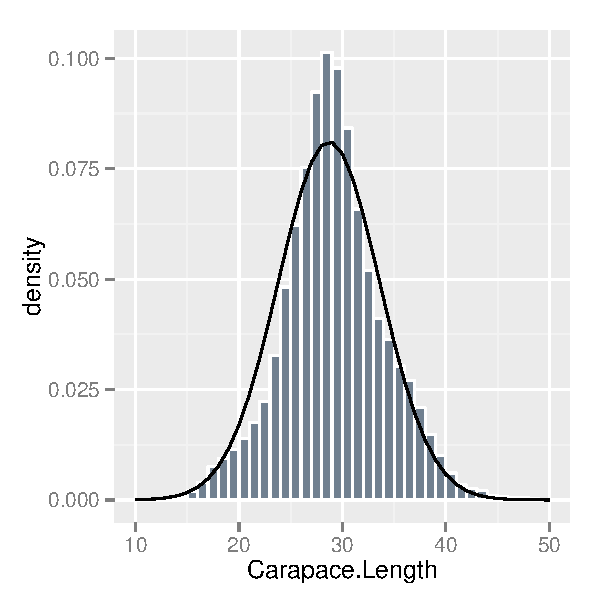
\includegraphics[width=\maxwidth]{figure/unnamed-chunk-7-1} \caption[Proportion of Nephrops catch retained per haul with fitted multinomial model and associated re-sampled intervals]{Proportion of Nephrops catch retained per haul with fitted multinomial model and associated re-sampled intervals. Null hypothesis of equal retention is displayed as the dashed line at 0.25.}\label{fig:unnamed-chunk-7}
\end{figure}


\end{knitrout}

\subsection{Including weight as a covariate}
Make a row per observation and merge with the weight data

\begin{knitrout}\footnotesize
\definecolor{shadecolor}{rgb}{0.969, 0.969, 0.969}\color{fgcolor}\begin{kframe}
\begin{alltt}
\hlcom{## get a row per length measurement (raise them also)}
\hlstd{n} \hlkwb{<-} \hlkwd{nrow}\hlstd{(neph.dat)}

\hlcom{##neph.dat2 <- neph.dat[rep(1:n, times = }
\hlcom{##                          round(neph.dat$COUNT/neph.dat$SUBSRATIO, 0)), ]}

\hlcom{## Note: no raising here}
\hlcom{##neph.dat2 <- neph.dat[rep(1:n, times = neph.dat$COUNT), ]}

\hlstd{weight.dat} \hlkwb{<-} \hlkwd{read.xls}\hlstd{(}\hlstr{"../data/Celtic Warrior Diamond mesh July 2014 Celtic Sea.xls"}\hlstd{,}
                       \hlkwc{sheet} \hlstd{=} \hlstr{"Weights"}\hlstd{,}
                       \hlkwc{stringsAsFactors} \hlstd{=} \hlnum{FALSE}\hlstd{)}

\hlcom{## Show the first 2 rows}
\hlkwd{head}\hlstd{(weight.dat,} \hlnum{2}\hlstd{)}
\end{alltt}
\begin{verbatim}
##         Date Haul.. Compartment Mesh.Size Species Total.weight..kg.
## 1 2014-07-19      1       TEST1      90mm    Bulk             26.28
## 2 2014-07-19      1       TEST1      90mm Haddock              0.38
##   Sbsample.weight..kg.
## 1                     
## 2
\end{verbatim}
\begin{alltt}
\hlcom{## create a new "HAUL" variable for the merge}
\hlstd{weight.dat}\hlopt{$}\hlstd{HAUL} \hlkwb{<-} \hlkwd{paste}\hlstd{(}\hlstr{"H"}\hlstd{, weight.dat}\hlopt{$}\hlstd{Haul..,} \hlkwc{sep} \hlstd{=}\hlstr{""}\hlstd{)}

\hlcom{## re-name total weight column}
\hlkwd{names}\hlstd{(weight.dat)[}\hlkwd{names}\hlstd{(weight.dat)} \hlopt{==} \hlstr{"Total.weight..kg."}\hlstd{]} \hlkwb{<-} \hlstr{"Total.Weight"}

\hlstd{weight.dat} \hlkwb{<-} \hlkwd{subset}\hlstd{(weight.dat, Species} \hlopt{==} \hlstr{"Bulk"}\hlstd{)}


\hlcom{## melt the data frame}
\hlstd{weight.melt} \hlkwb{<-} \hlkwd{melt}\hlstd{(weight.dat[,} \hlkwd{c}\hlstd{(}\hlstr{"HAUL"}\hlstd{,} \hlstr{"Mesh.Size"}\hlstd{,} \hlstr{"Total.Weight"}\hlstd{)],}
                  \hlkwc{id} \hlstd{=} \hlkwd{c}\hlstd{(}\hlstr{"Mesh.Size"}\hlstd{,} \hlstr{"HAUL"}\hlstd{))}

\hlcom{## re-form the dataframe in required format }
\hlstd{weight.cast} \hlkwb{<-} \hlkwd{cast}\hlstd{(weight.melt, HAUL} \hlopt{~} \hlstd{Mesh.Size}  \hlopt{+} \hlstd{variable)}
\hlstd{weight.cast} \hlkwb{<-} \hlstd{weight.cast[}\hlkwd{order}\hlstd{(weight.cast}\hlopt{$}\hlstd{HAUL), ]}
\hlstd{weight.cast[}\hlkwd{is.na}\hlstd{(weight.cast)]} \hlkwb{<-} \hlnum{0}

\hlcom{## show the first few rows}
\hlkwd{head}\hlstd{(weight.cast,} \hlnum{2}\hlstd{)}
\end{alltt}
\begin{verbatim}
##   HAUL 100mm_Total.Weight 70mm_Total.Weight 80mm_Total.Weight
## 1   H1              29.64             26.76             22.56
## 2  H10              52.00             50.40             60.10
##   90mm_Total.Weight
## 1             26.28
## 2             47.50
\end{verbatim}
\begin{alltt}
\hlstd{weight.cast}\hlopt{$}\hlstd{fHAUL} \hlkwb{<-} \hlkwd{factor}\hlstd{(weight.cast}\hlopt{$}\hlstd{HAUL)}

\hlkwd{names}\hlstd{(weight.cast)[}\hlkwd{grep}\hlstd{(}\hlstr{"^[0-9]"}\hlstd{,} \hlkwd{names}\hlstd{(weight.cast))]} \hlkwb{<-} \hlkwd{paste}\hlstd{(}\hlstr{"mesh."}\hlstd{,} \hlkwd{names}\hlstd{(weight.cast)[}\hlkwd{grep}\hlstd{(}\hlstr{"^[0-9]"}\hlstd{,} \hlkwd{names}\hlstd{(weight.cast))],} \hlkwc{sep} \hlstd{=} \hlstr{""}\hlstd{)}

\hlcom{## merge nephrops length and total bulk weight data}
\hlstd{neph.dat3} \hlkwb{<-} \hlkwd{merge}\hlstd{(neph.cast,}
                   \hlstd{weight.cast,}
                   \hlkwc{by} \hlstd{=} \hlkwd{c}\hlstd{(}\hlstr{"fHAUL"}\hlstd{),}
                   \hlkwc{sort} \hlstd{=} \hlnum{FALSE}
                   \hlstd{)}

\hlstd{max.length} \hlkwb{<-} \hlkwd{max}\hlstd{(neph.dat3}\hlopt{$}\hlstd{Carapace.Length)}
\hlstd{neph.dat3}\hlopt{$}\hlstd{prop.Carapace.Length} \hlkwb{<-} \hlstd{neph.dat3}\hlopt{$}\hlstd{Carapace.Length}\hlopt{/}\hlstd{max.length}
\hlstd{neph.dat3}\hlopt{$}\hlstd{prop.Carapace.Length2} \hlkwb{<-} \hlstd{neph.dat3}\hlopt{$}\hlstd{prop.Carapace.Length}\hlopt{^}\hlnum{2}
\hlstd{neph.dat3}\hlopt{$}\hlstd{prop.Carapace.Length3} \hlkwb{<-} \hlstd{neph.dat3}\hlopt{$}\hlstd{prop.Carapace.Length}\hlopt{^}\hlnum{3}
\hlstd{neph.dat3}\hlopt{$}\hlstd{prop.Carapace.Length4} \hlkwb{<-} \hlstd{neph.dat3}\hlopt{$}\hlstd{prop.Carapace.Length}\hlopt{^}\hlnum{4}
\end{alltt}
\end{kframe}
\end{knitrout}

Include weight in the fit

\begin{knitrout}\footnotesize
\definecolor{shadecolor}{rgb}{0.969, 0.969, 0.969}\color{fgcolor}\begin{kframe}
\begin{alltt}
\hlcom{## compare two ways of writing same model}

\hlcom{## in matrix format, as before except without offset for the moment}
\hlstd{mnom.length.matrix} \hlkwb{<-} \hlkwd{multinom}\hlstd{(}\hlkwd{as.matrix}\hlstd{(neph.dat3[,} \hlkwd{c}\hlstd{(}\hlstr{"70mm_COUNT"}\hlstd{,} \hlstr{"80mm_COUNT"}\hlstd{,} \hlstr{"90mm_COUNT"}\hlstd{,} \hlstr{"100mm_COUNT"}\hlstd{)])} \hlopt{~}
                               \hlstd{prop.Carapace.Length} \hlopt{+}
                               \hlstd{prop.Carapace.Length2} \hlopt{+}
                               \hlstd{prop.Carapace.Length3,}
                               \hlcom{##offset(offset.mat), }
                               \hlkwc{data} \hlstd{= neph.dat3)}
\end{alltt}
\begin{verbatim}
## # weights:  20 (12 variable)
## initial  value 65846.209564 
## iter  10 value 65594.036234
## iter  20 value 65560.638668
## final  value 65558.314009 
## converged
\end{verbatim}
\begin{alltt}
\hlcom{## take a look at the residuals by bulk weight}
\hlkwd{plot}\hlstd{(neph.dat3[,} \hlkwd{c}\hlstd{(}\hlstr{"mesh.70mm_Total.Weight"}\hlstd{,} \hlstr{"mesh.80mm_Total.Weight"}\hlstd{,} \hlstr{"mesh.90mm_Total.Weight"}\hlstd{,} \hlstr{"mesh.100mm_Total.Weight"}\hlstd{)])}
\end{alltt}
\end{kframe}
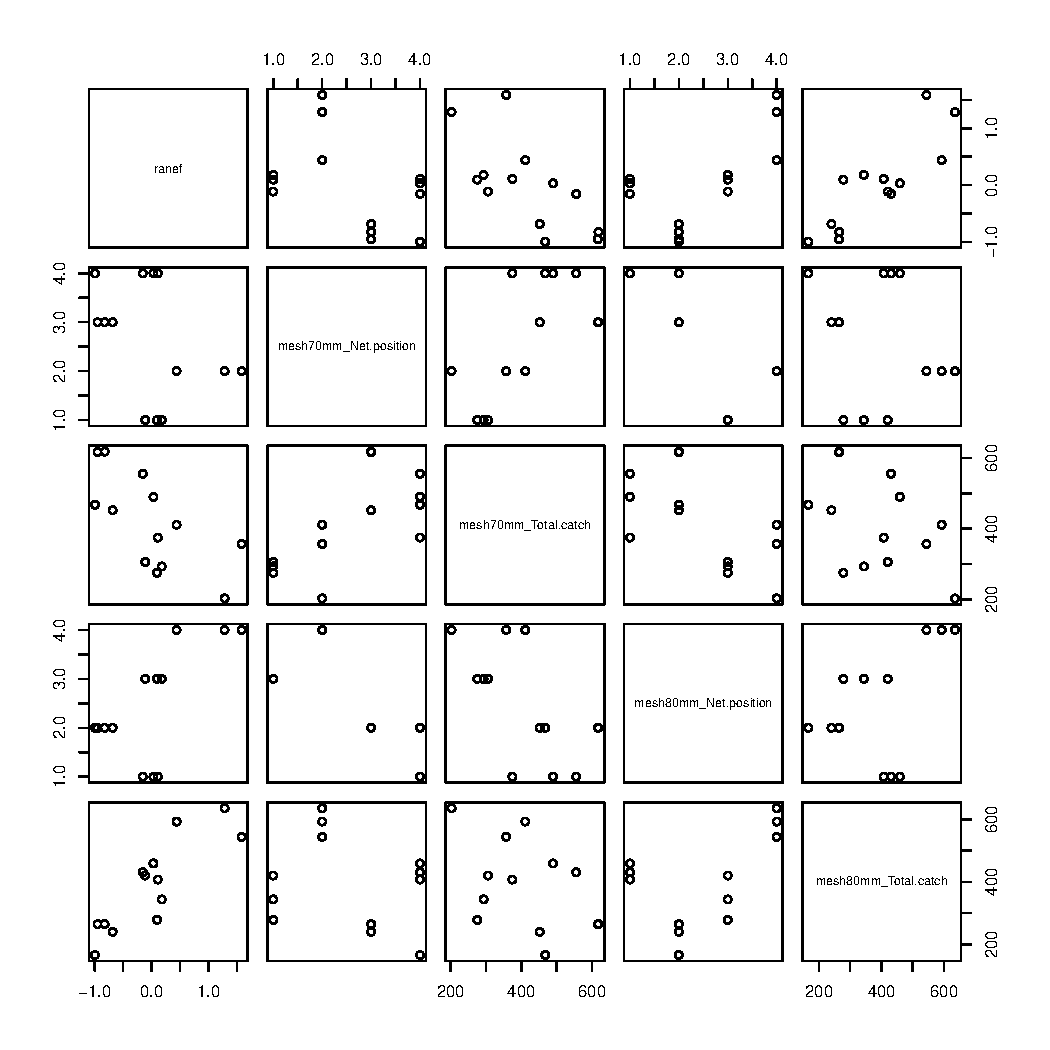
\includegraphics[width=\maxwidth]{figure/unnamed-chunk-9-1} 
\begin{kframe}\begin{alltt}
\hlcom{## very strong correlation in the counts}
\hlkwd{round}\hlstd{(}\hlkwd{cor}\hlstd{(neph.dat3[,} \hlkwd{c}\hlstd{(}\hlstr{"mesh.70mm_Total.Weight"}\hlstd{,} \hlstr{"mesh.80mm_Total.Weight"}\hlstd{,} \hlstr{"mesh.90mm_Total.Weight"}\hlstd{,} \hlstr{"mesh.100mm_Total.Weight"}\hlstd{)]),} \hlnum{3}\hlstd{)}
\end{alltt}
\begin{verbatim}
##                         mesh.70mm_Total.Weight mesh.80mm_Total.Weight
## mesh.70mm_Total.Weight                   1.000                  0.953
## mesh.80mm_Total.Weight                   0.953                  1.000
## mesh.90mm_Total.Weight                   0.927                  0.951
## mesh.100mm_Total.Weight                  0.882                  0.948
##                         mesh.90mm_Total.Weight mesh.100mm_Total.Weight
## mesh.70mm_Total.Weight                   0.927                   0.882
## mesh.80mm_Total.Weight                   0.951                   0.948
## mesh.90mm_Total.Weight                   1.000                   0.927
## mesh.100mm_Total.Weight                  0.927                   1.000
\end{verbatim}
\begin{alltt}
\hlcom{## resids versus weights}
\hlkwd{qplot}\hlstd{(neph.dat3[,} \hlkwd{c}\hlstd{(}\hlstr{"mesh.70mm_Total.Weight"}\hlstd{)],} \hlkwd{resid}\hlstd{(mnom.length.matrix)[,}\hlnum{1}\hlstd{])} \hlopt{+} \hlkwd{geom_smooth}\hlstd{()}
\end{alltt}


{\ttfamily\noindent\itshape\color{messagecolor}{\#\# geom\_smooth: method="{}auto"{} and size of largest group is <1000, so using loess. Use 'method = x' to change the smoothing method.}}\end{kframe}
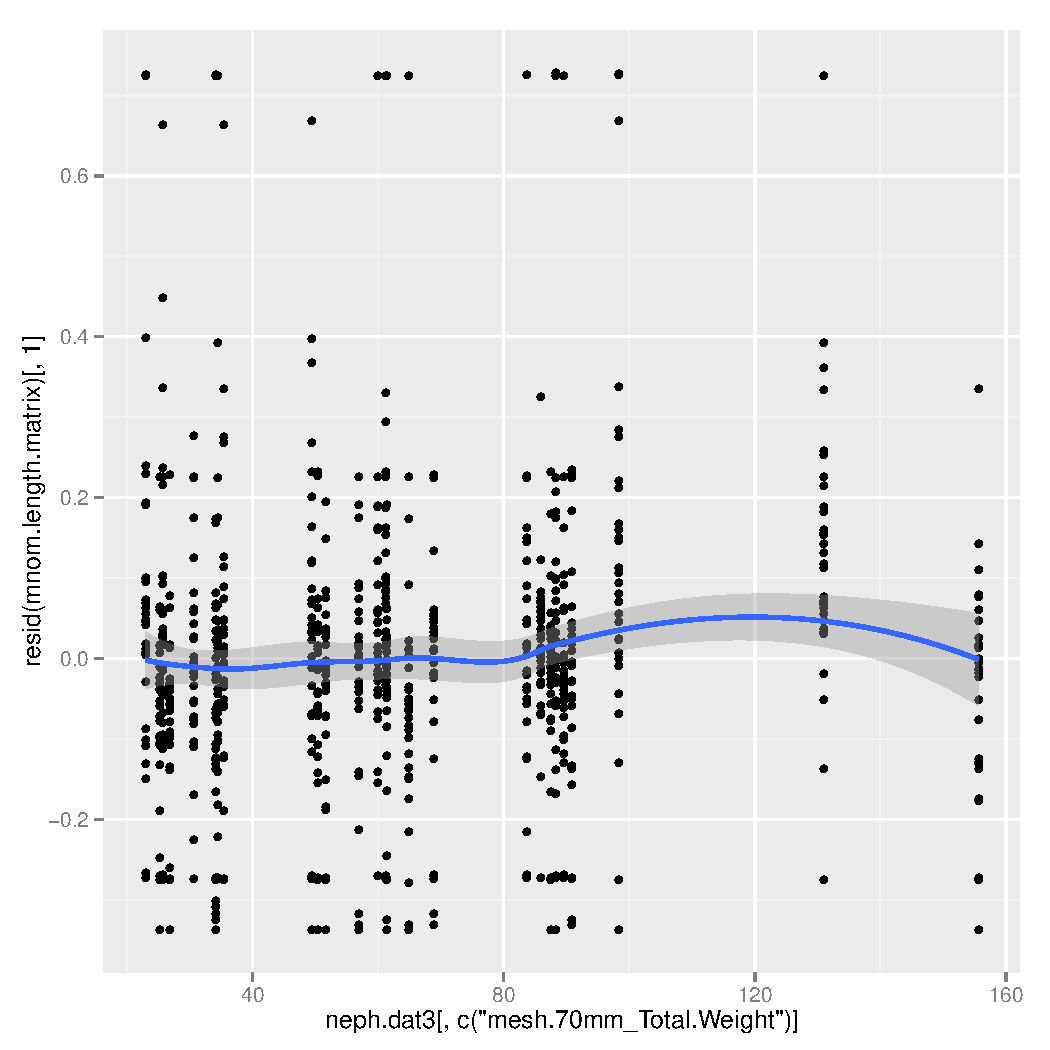
\includegraphics[width=\maxwidth]{figure/unnamed-chunk-9-2} 
\begin{kframe}\begin{alltt}
\hlkwd{qplot}\hlstd{(neph.dat3[,} \hlkwd{c}\hlstd{(}\hlstr{"mesh.80mm_Total.Weight"}\hlstd{)],} \hlkwd{resid}\hlstd{(mnom.length.matrix)[,}\hlnum{2}\hlstd{])} \hlopt{+} \hlkwd{geom_smooth}\hlstd{()}
\end{alltt}


{\ttfamily\noindent\itshape\color{messagecolor}{\#\# geom\_smooth: method="{}auto"{} and size of largest group is <1000, so using loess. Use 'method = x' to change the smoothing method.}}\end{kframe}
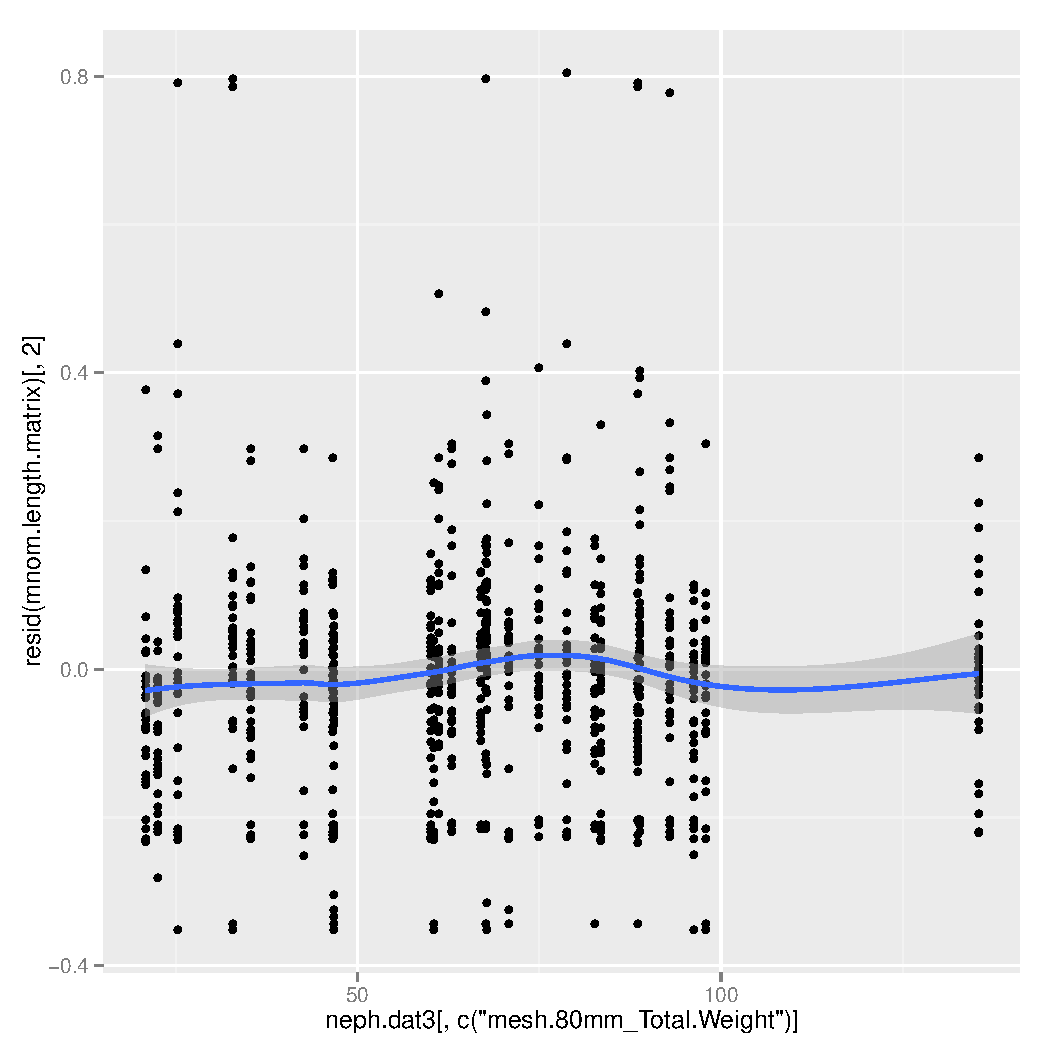
\includegraphics[width=\maxwidth]{figure/unnamed-chunk-9-3} 
\begin{kframe}\begin{alltt}
\hlkwd{qplot}\hlstd{(neph.dat3[,} \hlkwd{c}\hlstd{(}\hlstr{"mesh.90mm_Total.Weight"}\hlstd{)],} \hlkwd{resid}\hlstd{(mnom.length.matrix)[,}\hlnum{3}\hlstd{])} \hlopt{+} \hlkwd{geom_smooth}\hlstd{()}
\end{alltt}


{\ttfamily\noindent\itshape\color{messagecolor}{\#\# geom\_smooth: method="{}auto"{} and size of largest group is <1000, so using loess. Use 'method = x' to change the smoothing method.}}\end{kframe}
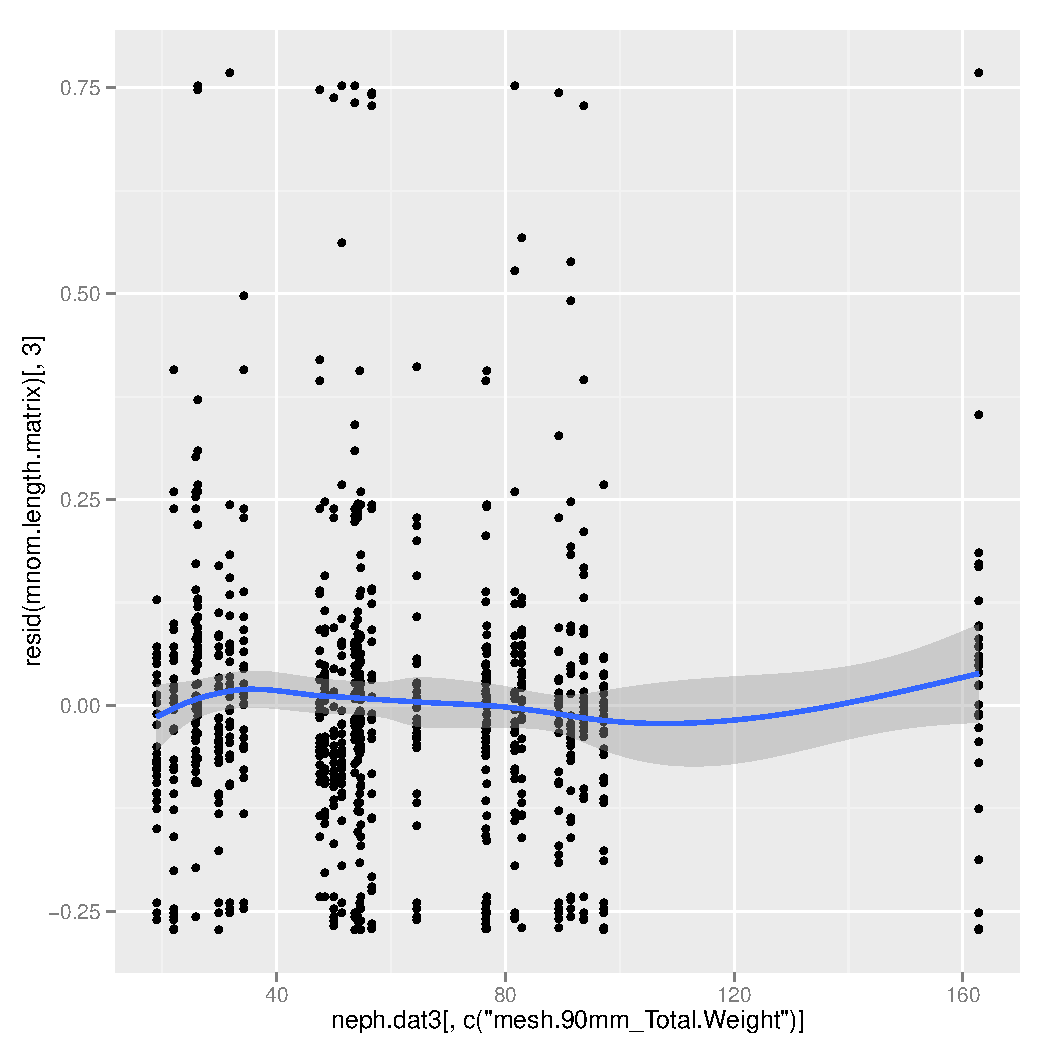
\includegraphics[width=\maxwidth]{figure/unnamed-chunk-9-4} 
\begin{kframe}\begin{alltt}
\hlkwd{qplot}\hlstd{(neph.dat3[,} \hlkwd{c}\hlstd{(}\hlstr{"mesh.100mm_Total.Weight"}\hlstd{)],} \hlkwd{resid}\hlstd{(mnom.length.matrix)[,}\hlnum{4}\hlstd{])} \hlopt{+} \hlkwd{geom_smooth}\hlstd{()}
\end{alltt}


{\ttfamily\noindent\itshape\color{messagecolor}{\#\# geom\_smooth: method="{}auto"{} and size of largest group is <1000, so using loess. Use 'method = x' to change the smoothing method.}}\end{kframe}
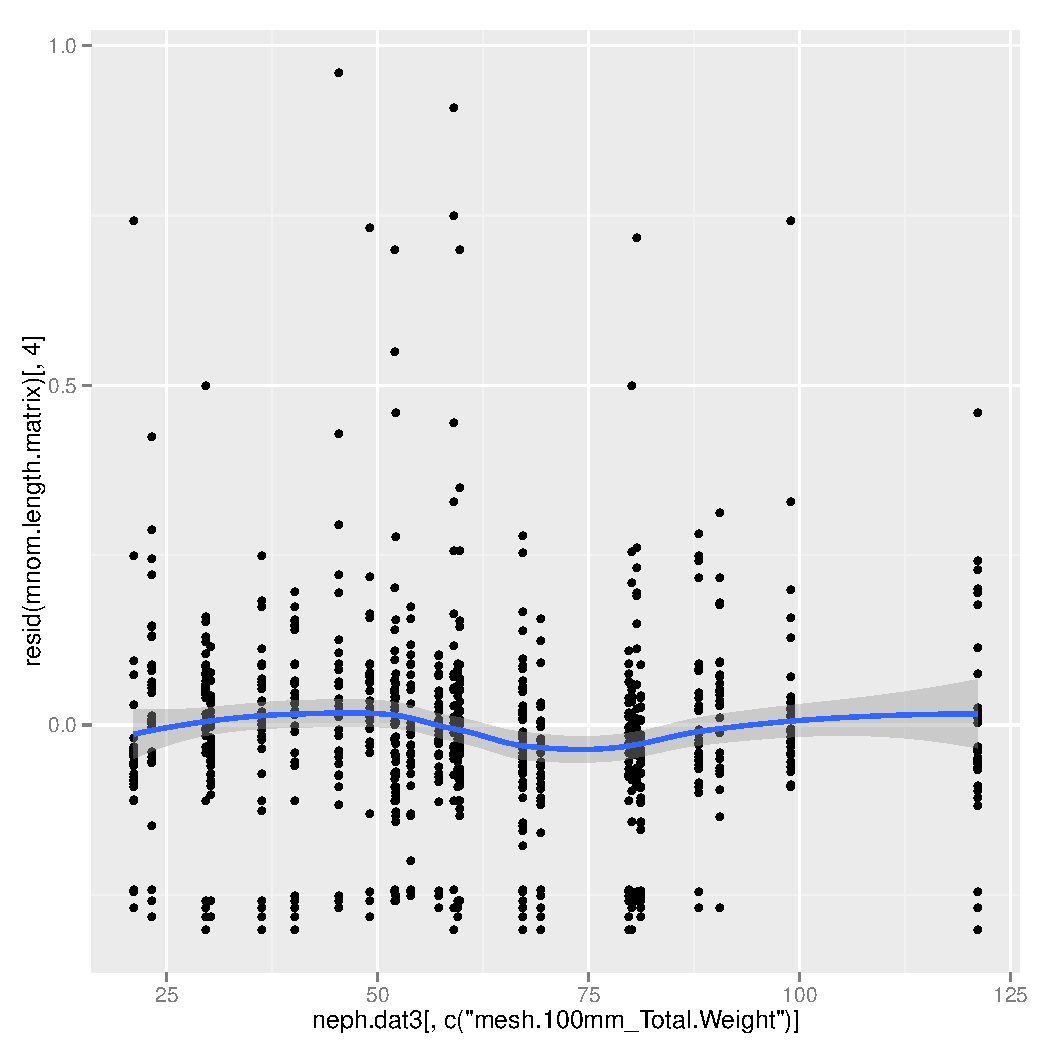
\includegraphics[width=\maxwidth]{figure/unnamed-chunk-9-5} 
\begin{kframe}\begin{alltt}
\hlcom{## include bulk weight in wide format model, note only including one of the}
\hlcom{## bulk weights as the explanatory}

\hlstd{neph.dat3}\hlopt{$}\hlstd{av.Total.Weight} \hlkwb{<-} \hlkwd{apply}\hlstd{(neph.dat3[,} \hlkwd{c}\hlstd{(}\hlstr{"mesh.70mm_Total.Weight"}\hlstd{,} \hlstr{"mesh.80mm_Total.Weight"}\hlstd{,} \hlstr{"mesh.90mm_Total.Weight"}\hlstd{,} \hlstr{"mesh.100mm_Total.Weight"}\hlstd{)],} \hlnum{1}\hlstd{, mean)}

\hlstd{mean.wt} \hlkwb{<-} \hlkwd{mean}\hlstd{(neph.dat3}\hlopt{$}\hlstd{av.Total.Weight)}

\hlstd{neph.dat3}\hlopt{$}\hlstd{av.Total.Weight.scaled} \hlkwb{<-} \hlstd{neph.dat3}\hlopt{$}\hlstd{av.Total.Weight} \hlopt{-} \hlstd{mean.wt}

\hlstd{mnom.length.bulk} \hlkwb{<-} \hlkwd{multinom}\hlstd{(}\hlkwd{as.matrix}\hlstd{(neph.dat3[,} \hlkwd{c}\hlstd{(}\hlstr{"70mm_COUNT"}\hlstd{,} \hlstr{"80mm_COUNT"}\hlstd{,} \hlstr{"90mm_COUNT"}\hlstd{,} \hlstr{"100mm_COUNT"}\hlstd{)])} \hlopt{~}
                             \hlstd{(}\hlkwd{poly}\hlstd{(av.Total.Weight.scaled,} \hlnum{2}\hlstd{)} \hlopt{+} \hlstd{prop.Carapace.Length)}\hlopt{^}\hlnum{2} \hlopt{+}
                             \hlstd{(}\hlkwd{poly}\hlstd{(av.Total.Weight.scaled,} \hlnum{2}\hlstd{)} \hlopt{+} \hlstd{prop.Carapace.Length2)}\hlopt{^}\hlnum{2} \hlopt{+}
                             \hlstd{(}\hlkwd{poly}\hlstd{(av.Total.Weight.scaled,} \hlnum{2}\hlstd{)} \hlopt{+} \hlstd{prop.Carapace.Length3)}\hlopt{^}\hlnum{2}\hlstd{,}
                             \hlcom{##offset(offset.mat),}
                             \hlkwc{data} \hlstd{= neph.dat3)}
\end{alltt}
\begin{verbatim}
## # weights:  52 (36 variable)
## initial  value 65846.209564 
## iter  10 value 65578.319726
## iter  20 value 65497.714497
## iter  30 value 65463.674596
## iter  40 value 65455.587103
## iter  50 value 65454.225846
## iter  60 value 65453.755984
## final  value 65453.493336 
## converged
\end{verbatim}
\begin{alltt}
\hlcom{## cut the weights here also}
\hlstd{wt.brks} \hlkwb{<-} \hlkwd{c}\hlstd{(}\hlnum{0}\hlstd{,} \hlnum{44}\hlstd{,} \hlnum{90}\hlstd{,} \hlnum{Inf}\hlstd{)}

\hlstd{neph.dat3}\hlopt{$}\hlstd{cmesh.70mm_Total.Weight} \hlkwb{<-} \hlkwd{cut}\hlstd{(neph.dat3}\hlopt{$}\hlstd{mesh.70mm_Total.Weight,} \hlkwc{breaks} \hlstd{= wt.brks)}
\hlstd{neph.dat3}\hlopt{$}\hlstd{cmesh.80mm_Total.Weight} \hlkwb{<-} \hlkwd{cut}\hlstd{(neph.dat3}\hlopt{$}\hlstd{mesh.80mm_Total.Weight,} \hlkwc{breaks} \hlstd{= wt.brks)}
\hlstd{neph.dat3}\hlopt{$}\hlstd{cmesh.90mm_Total.Weight} \hlkwb{<-} \hlkwd{cut}\hlstd{(neph.dat3}\hlopt{$}\hlstd{mesh.90mm_Total.Weight,} \hlkwc{breaks} \hlstd{= wt.brks)}
\hlstd{neph.dat3}\hlopt{$}\hlstd{cmesh.100mm_Total.Weight} \hlkwb{<-} \hlkwd{cut}\hlstd{(neph.dat3}\hlopt{$}\hlstd{mesh.100mm_Total.Weight,} \hlkwc{breaks} \hlstd{= wt.brks)}

\hlstd{mnom.length.bulkc} \hlkwb{<-} \hlkwd{multinom}\hlstd{(}\hlkwd{as.matrix}\hlstd{(neph.dat3[,} \hlkwd{c}\hlstd{(}\hlstr{"70mm_COUNT"}\hlstd{,} \hlstr{"80mm_COUNT"}\hlstd{,} \hlstr{"90mm_COUNT"}\hlstd{,} \hlstr{"100mm_COUNT"}\hlstd{)])} \hlopt{~}
                              \hlstd{prop.Carapace.Length} \hlopt{+}
                              \hlstd{prop.Carapace.Length2} \hlopt{+}
                              \hlstd{prop.Carapace.Length3} \hlopt{+}
                              \hlcom{##}
                              \hlstd{cmesh.70mm_Total.Weight} \hlopt{+}
                              \hlstd{cmesh.80mm_Total.Weight} \hlopt{+}
                              \hlstd{cmesh.90mm_Total.Weight} \hlopt{+}
                              \hlstd{cmesh.100mm_Total.Weight,}
                              \hlcom{##offset(offset.mat),}
                              \hlkwc{data} \hlstd{= neph.dat3)}
\end{alltt}
\begin{verbatim}
## # weights:  52 (36 variable)
## initial  value 65846.209564 
## iter  10 value 65654.262307
## iter  20 value 65557.651822
## iter  30 value 65464.946065
## iter  40 value 65424.314033
## iter  50 value 65416.861080
## final  value 65416.844867 
## converged
\end{verbatim}
\begin{alltt}
\hlkwd{AIC}\hlstd{(mnom.length.matrix, mnom.length.bulk, mnom.length.bulk.order1, mnom.length.bulk.order2, mnom.length.bulk.order3, mnom.length.bulk.order3c, mnom.length.bulk.order3.nl)}
\end{alltt}


{\ttfamily\noindent\bfseries\color{errorcolor}{\#\# Error in lapply(list(object, ...), ll): object 'mnom.length.bulk.order1' not found}}\begin{alltt}
\hlcom{## INCLUDE HIGHER-ORDER CARAPACE LENGTH}
\end{alltt}
\end{kframe}
\end{knitrout}

Get predictions for low, medium and high catch weights

\begin{knitrout}\footnotesize
\definecolor{shadecolor}{rgb}{0.969, 0.969, 0.969}\color{fgcolor}\begin{kframe}
\begin{alltt}
\hlcom{## In the model we include weights by compartment}
\hlcom{## in the predictions we fix the weights to be equal so we can see the mesh effects}
\hlcom{## 'standardize for weight effects so we can investigate mesh effects'}

\hlcom{## low.med.high.bulk <- quantile(weight.dat[weight.dat$Species == "Bulk",]$Total.Weight,}
\hlcom{##                               p = c(0.1, 0.5, 0.9))}
\hlcom{## low.med.high.bulk}
\hlcom{## ## set high to 120kg}
\hlcom{## low.med.high.bulk[3] <- 120}

\hlcom{## get mean total weight per bin used for empirical}
\hlstd{low.med.high.bulk} \hlkwb{<-} \hlkwd{with}\hlstd{(neph.dat.bulk,} \hlkwd{tapply}\hlstd{(Total.Weight, cTotal.Weight, mean))}
\end{alltt}


{\ttfamily\noindent\bfseries\color{errorcolor}{\#\# Error in with(neph.dat.bulk, tapply(Total.Weight, cTotal.Weight, mean)): object 'neph.dat.bulk' not found}}\begin{alltt}
\hlstd{pred.df} \hlkwb{<-} \hlkwd{expand.grid}\hlstd{(}\hlkwc{Carapace.Length} \hlstd{= pred.length,}
                       \hlkwc{av.Total.Weight} \hlstd{= low.med.high.bulk)}
\end{alltt}


{\ttfamily\noindent\bfseries\color{errorcolor}{\#\# Error in expand.grid(Carapace.Length = pred.length, av.Total.Weight = low.med.high.bulk): object 'low.med.high.bulk' not found}}\begin{alltt}
\hlstd{pred.df}\hlopt{$}\hlstd{av.Total.Weight.scaled} \hlkwb{<-} \hlstd{pred.df}\hlopt{$}\hlstd{av.Total.Weight}\hlopt{-} \hlstd{mean.wt}
\end{alltt}


{\ttfamily\noindent\bfseries\color{errorcolor}{\#\# Error in `\$<-.data.frame`(`*tmp*`, "{}av.Total.Weight.scaled"{}, value = numeric(0)): replacement has 0 rows, data has 400}}\begin{alltt}
\hlcom{## pred.df$mesh.80mm_Total.Weight <- pred.df$mesh.70mm_Total.Weight}
\hlcom{## pred.df$mesh.90mm_Total.Weight <- pred.df$mesh.70mm_Total.Weight}
\hlcom{## pred.df$mesh.100mm_Total.Weight <- pred.df$mesh.70mm_Total.Weight}

\hlcom{## pred.df$cmesh.70mm_Total.Weight <- cut(pred.df$mesh.70mm_Total.Weight, breaks = wt.brks)}
\hlcom{## pred.df$cmesh.80mm_Total.Weight <- cut(pred.df$mesh.80mm_Total.Weight, breaks = wt.brks)}
\hlcom{## pred.df$cmesh.90mm_Total.Weight <- cut(pred.df$mesh.90mm_Total.Weight, breaks = wt.brks)}
\hlcom{## pred.df$cmesh.100mm_Total.Weight <- cut(pred.df$mesh.100mm_Total.Weight, breaks = wt.brks)}

\hlstd{pred.df}\hlopt{$}\hlstd{prop.Carapace.Length} \hlkwb{<-} \hlstd{pred.df}\hlopt{$}\hlstd{Carapace.Length}\hlopt{/}\hlstd{max.length}
\end{alltt}


{\ttfamily\noindent\bfseries\color{errorcolor}{\#\# Error in `\$<-.data.frame`(`*tmp*`, "{}prop.Carapace.Length"{}, value = numeric(0)): replacement has 0 rows, data has 400}}\begin{alltt}
\hlstd{pred.df}\hlopt{$}\hlstd{prop.Carapace.Length2} \hlkwb{<-} \hlstd{pred.df}\hlopt{$}\hlstd{prop.Carapace.Length}\hlopt{^}\hlnum{2}
\end{alltt}


{\ttfamily\noindent\bfseries\color{errorcolor}{\#\# Error in `\$<-.data.frame`(`*tmp*`, "{}prop.Carapace.Length2"{}, value = numeric(0)): replacement has 0 rows, data has 400}}\begin{alltt}
\hlstd{pred.df}\hlopt{$}\hlstd{prop.Carapace.Length3} \hlkwb{<-} \hlstd{pred.df}\hlopt{$}\hlstd{prop.Carapace.Length}\hlopt{^}\hlnum{3}
\end{alltt}


{\ttfamily\noindent\bfseries\color{errorcolor}{\#\# Error in `\$<-.data.frame`(`*tmp*`, "{}prop.Carapace.Length3"{}, value = numeric(0)): replacement has 0 rows, data has 400}}\begin{alltt}
\hlcom{## Need to re-define offset here!!}
\hlcom{## Better to set offset as cbind in data frames}
\hlcom{##offset.mat <- matrix(0, ncol = 4, nrow = dim(pred.df)[1])}

\hlcom{##mnom.pred <- predict(mnom.length.bulk.order3, newdata = pred.df, type = "prob")}
\hlstd{mnom.pred} \hlkwb{<-} \hlkwd{predict}\hlstd{(mnom.length.bulk,} \hlkwc{newdata} \hlstd{= pred.df,} \hlkwc{type} \hlstd{=} \hlstr{"prob"}\hlstd{)}
\end{alltt}


{\ttfamily\noindent\bfseries\color{errorcolor}{\#\# Error in poly(av.Total.Weight.scaled, 2, coefs = structure(list(alpha = c(2.59920094279836e-15, : object 'av.Total.Weight.scaled' not found}}\begin{alltt}
\hlstd{m} \hlkwb{<-} \hlkwd{dim}\hlstd{(mnom.pred)[}\hlnum{1}\hlstd{]}
\end{alltt}


{\ttfamily\noindent\bfseries\color{errorcolor}{\#\# Error in eval(expr, envir, enclos): object 'mnom.pred' not found}}\begin{alltt}
\hlstd{mnom.pred.df} \hlkwb{<-} \hlkwd{data.frame}\hlstd{(}
                  \hlkwc{Mesh.Size} \hlstd{=} \hlkwd{factor}\hlstd{(}\hlkwd{rep}\hlstd{(}\hlkwd{c}\hlstd{(}\hlstr{"70mm"}\hlstd{,} \hlstr{"80mm"}\hlstd{,} \hlstr{"90mm"}\hlstd{,} \hlstr{"100mm"}\hlstd{),}
                    \hlkwc{each} \hlstd{= m),} \hlkwc{levels} \hlstd{=} \hlkwd{c}\hlstd{(}\hlstr{"70mm"}\hlstd{,} \hlstr{"80mm"}\hlstd{,} \hlstr{"90mm"}\hlstd{,} \hlstr{"100mm"}\hlstd{)),}
                  \hlkwc{Carapace.Length} \hlstd{=} \hlkwd{rep}\hlstd{(pred.df}\hlopt{$}\hlstd{Carapace.Length,} \hlkwc{times} \hlstd{=} \hlnum{4}\hlstd{),}
                  \hlkwc{prop.Carapace.Length} \hlstd{=} \hlkwd{rep}\hlstd{(pred.df}\hlopt{$}\hlstd{prop.Carapace.Length,} \hlkwc{times} \hlstd{=} \hlnum{4}\hlstd{),}
                  \hlkwc{av.Total.Weight} \hlstd{=} \hlkwd{rep}\hlstd{(pred.df}\hlopt{$}\hlstd{av.Total.Weight,} \hlkwc{times} \hlstd{=} \hlnum{4}\hlstd{),}
                  \hlkwc{proportion} \hlstd{=} \hlkwd{c}\hlstd{(mnom.pred))}
\end{alltt}


{\ttfamily\noindent\bfseries\color{errorcolor}{\#\# Error in data.frame(Mesh.Size = factor(rep(c("{}70mm"{}, "{}80mm"{}, "{}90mm"{}, "{}100mm"{}), : object 'mnom.pred' not found}}\begin{alltt}
\hlstd{mnom.pred.df}\hlopt{$}\hlstd{Bulk.Weight} \hlkwb{<-}
  \hlkwd{ifelse}\hlstd{(mnom.pred.df}\hlopt{$}\hlstd{av.Total.Weight} \hlopt{==} \hlstd{low.med.high.bulk[}\hlnum{1}\hlstd{],} \hlstr{"Low (26kg)"}\hlstd{,}
         \hlkwd{ifelse}\hlstd{(mnom.pred.df}\hlopt{$}\hlstd{av.Total.Weight} \hlopt{==} \hlstd{low.med.high.bulk[}\hlnum{2}\hlstd{],} \hlstr{"Medium (60.5kg)"}\hlstd{,} \hlstr{"High (120kg)"}\hlstd{)}
         \hlstd{)}
\end{alltt}


{\ttfamily\noindent\bfseries\color{errorcolor}{\#\# Error in ifelse(mnom.pred.df\$av.Total.Weight == low.med.high.bulk[1], : object 'mnom.pred.df' not found}}\begin{alltt}
\hlstd{mnom.pred.df}\hlopt{$}\hlstd{Bulk.Weight} \hlkwb{<-} \hlkwd{factor}\hlstd{(mnom.pred.df}\hlopt{$}\hlstd{Bulk.Weight,}
                                   \hlkwc{levels} \hlstd{=} \hlkwd{c}\hlstd{(}\hlstr{"Low (26kg)"}\hlstd{,} \hlstr{"Medium (60.5kg)"}\hlstd{,} \hlstr{"High (120kg)"}\hlstd{))}
\end{alltt}


{\ttfamily\noindent\bfseries\color{errorcolor}{\#\# Error in factor(mnom.pred.df\$Bulk.Weight, levels = c("{}Low (26kg)"{}, "{}Medium (60.5kg)"{}, : object 'mnom.pred.df' not found}}\begin{alltt}
\hlstd{p} \hlopt{+} \hlkwd{geom_line}\hlstd{(}\hlkwc{data} \hlstd{= mnom.pred.df,}
              \hlkwd{aes}\hlstd{(}\hlkwc{x} \hlstd{= Carapace.Length,} \hlkwc{y} \hlstd{= proportion,}
                  \hlkwc{group} \hlstd{= Bulk.Weight,}
                  \hlkwc{colour} \hlstd{= Bulk.Weight))} \hlopt{+}
  \hlkwd{scale_colour_manual}\hlstd{(}\hlkwc{values}\hlstd{=}\hlkwd{c}\hlstd{(}\hlstr{"#619CFF"}\hlstd{,} \hlstr{"#00BA38"}\hlstd{,} \hlstr{"#FF0000"}\hlstd{))} \hlopt{+}
\hlcom{##scale_colour_manual(values = c("blue", "green", "red")) +}
\hlkwd{geom_hline}\hlstd{(}\hlkwd{aes}\hlstd{(}\hlkwc{yintercept} \hlstd{=} \hlnum{0.25}\hlstd{),} \hlkwc{linetype} \hlstd{=} \hlstr{"dashed"}\hlstd{)} \hlopt{+}
  \hlkwd{geom_vline}\hlstd{(}\hlkwd{aes}\hlstd{(}\hlkwc{xintercept} \hlstd{=} \hlnum{25}\hlstd{),} \hlkwc{linetype} \hlstd{=} \hlstr{"dashed"}\hlstd{)}
\end{alltt}


{\ttfamily\noindent\bfseries\color{errorcolor}{\#\# Error in do.call("{}layer"{}, list(mapping = mapping, data = data, stat = stat, : object 'mnom.pred.df' not found}}\end{kframe}
\end{knitrout}

\begin{knitrout}\footnotesize
\definecolor{shadecolor}{rgb}{0.969, 0.969, 0.969}\color{fgcolor}\begin{kframe}
\begin{alltt}
\hlcom{## draw empirical lines}
\hlcom{## bin the weights}
\hlstd{neph.dat.bulk} \hlkwb{<-}  \hlkwd{merge}\hlstd{(neph.dat, weight.dat)}

\hlstd{neph.dat.bulk}\hlopt{$}\hlstd{cTotal.Weight} \hlkwb{<-} \hlkwd{cut}\hlstd{(neph.dat.bulk}\hlopt{$}\hlstd{Total.Weight,} \hlkwc{breaks} \hlstd{= wt.brks)}
\hlcom{##neph.dat.bulk$cTotal.Weight <- 1}

\hlcom{## RAISING NOT INCLUDED UNTIL OFFSET INCLUDED}
\hlcom{##neph.dat.bulk$rCOUNT <- with(neph.dat.bulk, COUNT/SUBSRATIO)}
\hlstd{neph.dat.bulk}\hlopt{$}\hlstd{rCOUNT} \hlkwb{<-} \hlkwd{with}\hlstd{(neph.dat.bulk, COUNT)}

\hlstd{count.array} \hlkwb{<-} \hlkwd{with}\hlstd{(neph.dat.bulk,} \hlkwd{tapply}\hlstd{(rCOUNT,} \hlkwd{list}\hlstd{(cTotal.Weight, Carapace.Length, Mesh.Size), sum))}

\hlstd{count.array[}\hlkwd{is.na}\hlstd{(count.array)]} \hlkwb{<-} \hlnum{0}

\hlstd{prop.array} \hlkwb{<-} \hlkwd{prop.table}\hlstd{(count.array,} \hlkwd{c}\hlstd{(}\hlnum{1}\hlstd{,}\hlnum{2}\hlstd{))}

\hlstd{prop.df} \hlkwb{<-} \hlkwd{expand.grid}\hlstd{(}\hlkwc{Total.Weight} \hlstd{=} \hlkwd{dimnames}\hlstd{(prop.array)[[}\hlnum{1}\hlstd{]],}
                       \hlkwc{Carapace.Length} \hlstd{=} \hlkwd{dimnames}\hlstd{(prop.array)[[}\hlnum{2}\hlstd{]],}
                       \hlkwc{Mesh.Size} \hlstd{=} \hlkwd{dimnames}\hlstd{(prop.array)[[}\hlnum{3}\hlstd{]],}
                       \hlkwc{stringsAsFactors} \hlstd{=} \hlnum{FALSE}\hlstd{)}

\hlstd{prop.df}\hlopt{$}\hlstd{empirical.prop} \hlkwb{<-} \hlnum{NA}
\hlstd{prop.df}\hlopt{$}\hlstd{rCOUNT} \hlkwb{<-} \hlnum{NA}

\hlkwa{for}\hlstd{(i} \hlkwa{in} \hlnum{1}\hlopt{:}\hlkwd{dim}\hlstd{(prop.df)[}\hlnum{1}\hlstd{])\{}
  \hlcom{## proportion}
  \hlstd{prop.df}\hlopt{$}\hlstd{empirical.prop[i]} \hlkwb{<-} \hlstd{prop.array[prop.df}\hlopt{$}\hlstd{Total.Weight[i],}
                                          \hlstd{prop.df}\hlopt{$}\hlstd{Carapace.Length[i],}
                                          \hlstd{prop.df}\hlopt{$}\hlstd{Mesh.Size[i]}
                                          \hlstd{]}
  \hlcom{## count}
  \hlstd{prop.df}\hlopt{$}\hlstd{rCOUNT[i]} \hlkwb{<-} \hlstd{count.array[prop.df}\hlopt{$}\hlstd{Total.Weight[i],}
                                   \hlstd{prop.df}\hlopt{$}\hlstd{Carapace.Length[i],}
                                   \hlstd{prop.df}\hlopt{$}\hlstd{Mesh.Size[i]}
                                   \hlstd{]}
\hlstd{\}}

\hlstd{prop.df}\hlopt{$}\hlstd{Bulk.Weight} \hlkwb{<-} \hlkwd{ifelse}\hlstd{(prop.df}\hlopt{$}\hlstd{Total.Weight} \hlopt{==} \hlstr{"(0,44]"}\hlstd{,} \hlstr{"Low (26kg)"}\hlstd{,}
                              \hlkwd{ifelse}\hlstd{(prop.df}\hlopt{$}\hlstd{Total.Weight} \hlopt{==} \hlstr{"(44,90]"}\hlstd{,} \hlstr{"Medium (60.5kg)"}\hlstd{,} \hlstr{"High (120kg)"}\hlstd{)}
                              \hlstd{)}

\hlstd{prop.df}\hlopt{$}\hlstd{Carapace.Length} \hlkwb{<-} \hlkwd{as.numeric}\hlstd{(prop.df}\hlopt{$}\hlstd{Carapace.Length)}

\hlstd{prop.df}\hlopt{$}\hlstd{Mesh.Size} \hlkwb{<-} \hlkwd{factor}\hlstd{(prop.df}\hlopt{$}\hlstd{Mesh.Size,} \hlkwc{levels} \hlstd{=} \hlkwd{c}\hlstd{(}\hlstr{"70mm"}\hlstd{,} \hlstr{"80mm"}\hlstd{,} \hlstr{"90mm"}\hlstd{,}\hlstr{"100mm"}\hlstd{))}

\hlcom{## empirical versus modelled}

\hlcom{##pdf("../tex/figures/")}
\hlkwd{ggplot}\hlstd{(prop.df,} \hlkwd{aes}\hlstd{(}\hlkwc{x} \hlstd{= Carapace.Length,} \hlkwc{y} \hlstd{= empirical.prop,}
                \hlkwc{group} \hlstd{= Bulk.Weight,}
                \hlkwc{colour} \hlstd{= Bulk.Weight))} \hlopt{+}
  \hlkwd{geom_point}\hlstd{(}\hlkwd{aes}\hlstd{(}\hlkwc{size} \hlstd{=} \hlkwd{log}\hlstd{(rCOUNT)),} \hlkwc{linetype} \hlstd{=} \hlstr{"dashed"}\hlstd{,} \hlkwc{alpha} \hlstd{=} \hlnum{0.5}\hlstd{)} \hlopt{+}
  \hlkwd{facet_wrap}\hlstd{(}\hlopt{~} \hlstd{Mesh.Size)} \hlopt{+}
  \hlkwd{geom_line}\hlstd{(}\hlkwc{data} \hlstd{= mnom.pred.df,} \hlkwd{aes}\hlstd{(}\hlkwc{x} \hlstd{= Carapace.Length,} \hlkwc{y} \hlstd{= proportion,}
              \hlkwc{group} \hlstd{= Bulk.Weight,}
              \hlkwc{colour} \hlstd{= Bulk.Weight))} \hlopt{+}
  \hlkwd{geom_hline}\hlstd{(}\hlkwd{aes}\hlstd{(}\hlkwc{yintercept} \hlstd{=} \hlnum{0.25}\hlstd{),} \hlkwc{linetype} \hlstd{=} \hlstr{"dashed"}\hlstd{)} \hlopt{+}
  \hlkwd{geom_vline}\hlstd{(}\hlkwd{aes}\hlstd{(}\hlkwc{xintercept} \hlstd{=} \hlnum{25}\hlstd{),} \hlkwc{linetype} \hlstd{=} \hlstr{"dashed"}\hlstd{)}
\end{alltt}


{\ttfamily\noindent\bfseries\color{errorcolor}{\#\# Error in do.call("{}layer"{}, list(mapping = mapping, data = data, stat = stat, : object 'mnom.pred.df' not found}}\end{kframe}
\end{knitrout}


\bibliography{../../../../misc/epif_bibliography}
\bibliographystyle{../../../../misc/cjfas}
\end{document}

